\documentclass[a4paper,11pt]{article}
\usepackage{cmap}
\usepackage{polski}
\usepackage[T1]{fontenc}
\usepackage[utf8]{inputenc}
\usepackage{listings}
\usepackage{graphicx}  
\graphicspath{ {C:/Users/jankl/} }



\title{Sprawozdanie nr 2}
\author{Łukasz Szumilas}
\date{Zajęcia: 5 listopad 2018}

\begin{document}
  \begin{center}\Large
    Grafika Komputerowa i Komunikacja Człowiek-Komputer
  \end{center}
  \hrule
  {\let\newpage\relax\maketitle}
  \hrule


  \section{Omówienie tematu}
   Celem zajęć było wprowadzenie w zagadnienia modelowania i wizualizacji scen 3D z wykorzystaniem biblioteki OpenGL z rozszerzeniem GLUT. Zaimplementowane w środowisku Visual Studio przykłady pokazywały jak w układzie współrzędnych trójwymiarowych wykonuje się transformacje obiektów oraz jak na podstawie równań parametrycznych można stworzyć  model  danego obiektu 3D. 
\\\indent Aby móc konstruować modele 3D najpierw trzeba było zdefiniować i narysować układ współrzędnych w rzutowaniu ortograficznym. \textit{(kod 1, Rysunek 1)} W rzucie tym płaszczyzna na której powstawał obraz, była równoległa do płaszczyzny tworzonej przez osie \textit{x} i \textit{y}, a proste rzutowania biegły równoległe do osi \textit{z}. Na laboratorium w użytych przykładach z tego rzutowania oś \textit{z} nie jest widoczna.  
\\\indent Dla szybkiego efektu wizualizacji w jaki sposób zachowują się obiekty w zdefiniowanych współrzędnych użyty był gotowy kod rysujący imbryczek. \textit{(kod 2, Rysunek 2)}. Imbryk jako obiekt  asymetryczny dobrze nadaje się do śledzenia rezultatów zastosowanych transformacji, które trzeba było wykonać w następnym etapie. 
\\\indent Najlepszą formą przedstawienia transformacji jest macierz, dlatego wszystkie funkcje używane w OpenGL dotyczące przedstawienia obiektu w inny sposób wykorzystują rachunek macierzowy. Konkretne funkcje użyte na zajęciach to:              \\\\ \textit{glTranslated(TYP x, TYPE y, TYPE z)},
\\\textit{glRotated(TYPE angle, TYPE x, TYPE y, TYPE z,)},
\\\\gdzie pierwsza dotyczy przesunięcia obiektu wzdłuż osi a druga obrotu o daty kąt \textit{angle} także wokół wybranych osi. Transformacja obiektu została przedstawiona w  \textit{kodzie 3 i rysunku 3}.
\\W następnym etapie trzeba było zbudować własny model 3D. Obiektem miało być jajko, które miało powstać za pomocą wzorów definiujących chmurę punktów w trójwymiarowej płaszczyźnie
\\ (wzor ze strony: http://www.zsk.ict.pwr.wroc.pl)
  \begin{figure}[h!]
      \centering
      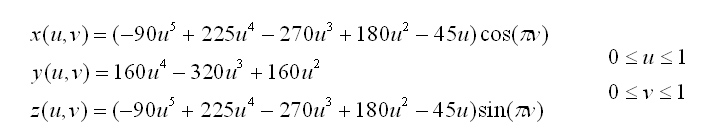
\includegraphics[width=1\textwidth,height=2.5cm]{wzor.png}
      \label{fig:zrzut1}
    \end{figure}
\\Chmura punktów (u,v) powstała w dwuwymiarowej tablicy \textbf{NxN}, gdzie\textbf{N} oznacza liczbę przedziałów jednostkowego kwadratu. Rezultat zmagań z tym zadaniem został przedstawiony w \textit{kodzie 4 i rysunku 4}

  \section{Omówienie kodu}
   \textbf{Kod 1}, po wywołaniu ukazuje się nam układ współrzędnych.  
{\small
\begin{lstlisting}[language=C++]

typedef float point3[3]; 
//zdefiniowane tablicy point3 typu float przechowujacej wspolrzedne

void Axes(void)
{
point3  x_min = {-5.0, 0.0, 0.0};
point3  x_max = { 5.0, 0.0, 0.0}; 
// poczatek i koniec obrazu osi x

point3  y_min = {0.0, -5.0, 0.0}; 
point3  y_max = {0.0,  5.0, 0.0};
// poczatek i koniec obrazu osi y

point3  z_min = {0.0, 0.0, -5.0};
point3  z_max = {0.0, 0.0,  5.0};
//  poczatek i koniec obrazu osi y
glColor3f(1.0f, 0.0f, 0.0f);  // kolor rysowania osi - czerwony
glBegin(GL_LINES); // rysowanie osi x
glVertex3fv(x_min);
glVertex3fv(x_max);
glEnd();

glColor3f(0.0f, 1.0f, 0.0f);  // kolor rysowania - zielony
glBegin(GL_LINES);  // rysowanie osi y

glVertex3fv(y_min);
glVertex3fv(y_max);                           
glEnd();

glColor3f(0.0f, 0.0f, 1.0f);  // kolor rysowania - niebieski
glBegin(GL_LINES); // rysowanie osi z

glVertex3fv(z_min);
glVertex3fv(z_max);
glEnd();

}
\end{lstlisting}
}
.\\
\textbf{Kod 2}, po wywołaniu funkcji \textit{Axes()} zmieniamy kolor rysowania i wywołujemy funkcję rysującą gotowy obiekt. 
{\small
\begin{lstlisting}[language=C++]
glColor3f(1.0f, 1.0f, 1.0f); // Ustawienie koloru rysowania
glutWireTeapot(3.0); // Imbryczek
\end{lstlisting}
}

.\\
\textbf{Kod 3}, użyty na końcu funkcji \textit{Axes()}.   
{\small
\begin{lstlisting}[language=C++]
glRotated(300, 1.0, 0.0, 0.0); // Obrot o 300 stopni wokol osi x
glTranslated(0.0, 3.0, 0.0);
f //przesuniecie obiektu o 3 jednostki w gore wzdloz osi y
\end{lstlisting}
}
.\\
\textbf{Kod 4}, najpierw trzeba było zdefiniować rodzaj zmiennych, które mogły przechowywać zarówno chmurę punktów jak i współrzędne dla każdego z tych punktów odwzorowane w trójwymiarowym układzie. Wskaźniki pomogły definiować rozmiar tablic w sposób dynamiczny, przez co łatwiej zmieniało się liczbę punktów, z których powstawało jajko.   
{\small
\begin{lstlisting}[language=C++]
point3 ***tabXYZ = new point3**[N];
point2 **UV = new point2*[N];
\end{lstlisting}
}
Funkcja \textit{Egg()} wywoływana była po narysowaniu współrzędnych i zmianie koloru rysowania na biały. 

{\small
\begin{lstlisting}[language=C++]
void Egg()
{
float numerU = 0;  //wspolrzedna U na kwadracie
float numerV = 0;  //wspolrzedna V na kwadracie
float distance = 1 / N;  
//podzial kwadratu jednostkowego na N przedzialow

for (int i = 0; i < N; i++)
{
tabXYZ[i] = new point3*[N];   //rozmiar tablicy XYZ
UV[i] = new point2[N];		 //rozmiar tablicy UV
	for (int j = 0; j < N; j++)
	{
		float u = numerU;
		float v = numerV;
		point2 a = { u,v };
		*UV[i][j] = *a;
	//obliczanie punktow X,Y,Z
float rownanieX = (-90 * pow(u, 5) + 225 * pow(u, 4) - 
270 * pow(u, 3) + 180 * pow(u, 2) - 45 * (u))*cos(3.14*(v));
float rownanieY = (160 * pow(u, 4) - 320 * pow(u, 3) + 160 * 
pow(u, 2));
float rownanieZ = (-90 * pow(u, 5) + 225 * pow(u, 4) - 
270 * pow(u, 3) + 180 * pow(u, 2) - 45 * (u))*sin(3.14*(v));

		point3 ej = { rownanieX, rownanieY, rownanieZ }; 
//przypisanie punktow do trojwymiarowej zmienne
		tabXYZ[i][j] = &ej;

		glBegin(GL_POINTS);		
//rysowanie jajka
			glVertex3fv(*tabXYZ[i][j]);   
		glEnd();

		numerV += distance;	
//nastepny punkt V w kwadracie  
	}
	numerU += distance;	
//nastepny punkt U w kwadracie  
	numerV = 0;
}
}
\end{lstlisting}
}

  \section{Rezultat prac}

    \begin{figure}[h!]
      \centering
      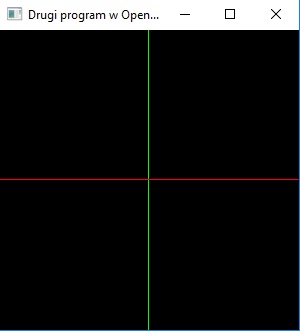
\includegraphics[width=0.6\textwidth,height=8cm]{ukladwsp.png}
      \caption{Układ współrzędnych}
      \label{fig:zrzut1}
    \end{figure}

    \begin{figure}[h!]
      \centering
      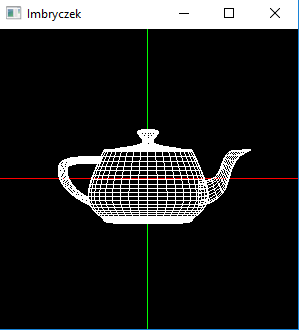
\includegraphics[width=0.6\textwidth,height=8cm]{imbryk.png}
      \caption{Imbryczek. Obiekt 3D w układzie współrzędnych}
      \label{fig:zrzut1}
    \end{figure}

    \begin{figure}[h!]
      \centering
      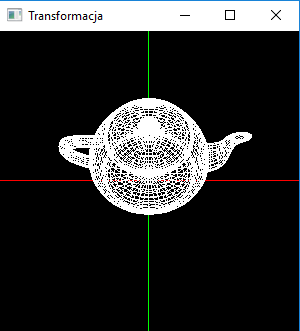
\includegraphics[width=0.6\textwidth,height=8cm]{transformacja.png}
      \caption{Imbryczek po transformacji}
      \label{fig:zrzut1}
    \end{figure}

    \begin{figure}[h!]
      \centering
      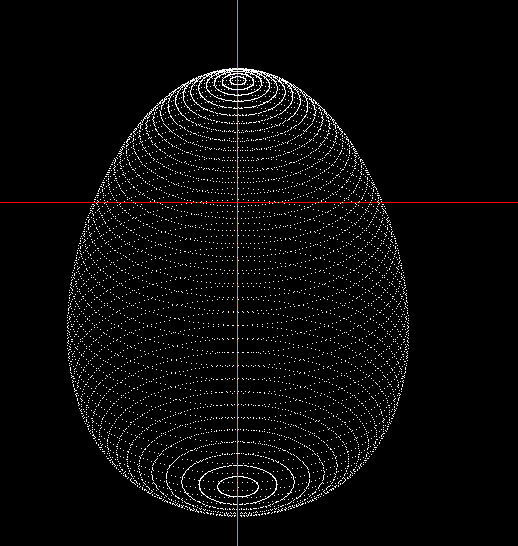
\includegraphics[width=0.6\textwidth,height=8cm]{jajco.png}
      \caption{Jajko po transformacji, chmura punktów}
      \label{fig:zrzut1}
    \end{figure}

\end{document}